\chapter{Conclusions and Outlook}
\label{sec:conclusions}
\chaptermark{Conclusions}

Two of the overarching goals behind the construction of the LHC and its detectors were to search for any evidence of the Standard Model Higgs boson and to look for any signs of new physics beyond the Standard Model. Behind the work of hundreds of collaborators and centuries of combined experience, the first goal was achieved. In Sec.~\ref{sec:discovery}, using the $H\rightarrow ZZ\rightarrow 4l$ decay channel over the first run of data for CMS, a Higgs boson near $m_{H}=125.6$ $\rm{GeV}$ was observed to $~7\sigma$ global significance. The matrix element methods outlined in Sec.~\ref{sec:pheno} were crucial to its discovery. The second goal of the LHC, observations that indicate new physics, are a bit more nuanced. At the time of writing, the LHC has yet to observe additional resonances that would be indicative of any theoretical extension of the Standard Model. However, we do have a Higgs boson. If its properties disagree with the expectations of the Standard Model, then particle physicists may have a sign of what the next development will be.

As shown in Sec.~\ref{sec:properties}, the $m_{H}=125.6$ $\rm{GeV}$ Higgs boson appears to match many of the expectations of the Standard Model. In Sec.~\ref{sec:HighMass}, no additional Higgs-like resonances were found in the high mass region. The spin-parity of the Higgs boson should be a spin-0 CP-even particle. Looking at the results of Sec.~\ref{sec:SpinParity}, any spin-1 or spin-2 model is excluded, many at $\geq3\sigma$. From Sec.~\ref{sec:SpinParity} and \ref{sec:OffShellAnom}, the fractional measurements of the anomalous $HVV$ couplings are all in agreement with what should be expected for the Standard Model Higgs boson given current statistical and theoretical limitations. Finally, the total width of the resonance, if anomalously large, would be a strong sign of new physics. But as calculated in Sec.~\ref{sec:WidthResults} and \ref{sec:OffShellAnom} using the combined on-shell and off-shell regions, the width is in agreement with Standard Model expectations. Indeed, when looking at the combination result from all decay channels in CMS, the Higgs boson's signal strength agrees with the predictions, even when split by decay mode as in Fig.~\ref{fig:CombHiggsDecay} or when split by production mode\footnote{There is an excess in $t\bar{t}H$ production, coming largely from $H\rightarrow \gamma\gamma$ and $H\rightarrow WW$.} as in Fig.~\ref{fig:CombHiggsProd}.

\begin{figure}[htbp]
\begin{center}
\includegraphics[width=.45\linewidth]{Conclusions/figures/sqr_mlz_ccc_mH125_decay.pdf}
\includegraphics[width=.45\linewidth]{Conclusions/figures/sqr_m6summary_fitmu.pdf}
\caption[Higgs Boson Signal Strength for CMS Combination Split by Decay Channel]{On left, signal strengths for the combination (vertical black line, with green $\pm1\sigma$ uncertainty bands) and split via subcombinations of bosonic ($H\rightarrow \gamma\gamma$, $H\rightarrow ZZ$, $H\rightarrow WW$) and fermionic ($H\rightarrow \tau\tau$, $H\rightarrow b\bar{b}$) decay modes with horizontal red bars for $\pm1\sigma$ uncertainty around best fit value. On right, deviations of the Higgs boson coupling to fermions and bosons are plotted. Particle masses are taken from \cite{Agashe:2014kda}. Both plots are from \cite{Khachatryan:2014jba}.}
\label{fig:CombHiggsDecay}
\end{center}
\end{figure}

\begin{figure}[htbp]
\begin{center}
\includegraphics[width=.45\linewidth]{Conclusions/figures/sqr_mlz_ccc_mH125_prod.pdf}
\includegraphics[width=.45\linewidth]{Conclusions/figures/sqr_rvrf_scan_2d_all_68.pdf}
\caption[Higgs Boson Signal Strength for CMS Combination Split by Production]{On left, signal strengths for the combination (vertical black line, with green $\pm1\sigma$ uncertainty bands) and split via subcombinations of tags for different production mechanisms (VBF, VH, $t\bar{t}H$, and Untagged) with horizontal red bars for $\pm1\sigma$ uncertainty around best fit value. On right, comparison of signal strength for bosonic ($\mu_{\rm VBF,VH}$) vs fermionic ($\mu_{\rm ggH,ttH}$) couplings split by decay channel, with a cross and $1\sigma$ contour for each decay channel plotted alongside the SM expectations (red and yellow diamond). Both plots are from \cite{Khachatryan:2014jba}.}
\label{fig:CombHiggsProd}
\end{center}
\end{figure}

However, just because results currently agree with the expectations of the Standard Model does not imply that this Higgs boson is The Higgs Boson. The second run of the LHC at $13$ $\rm{TeV}$ is about to begin physics runs, do we have any expectations of what sensitivity we can reach in these property measurements?

For the total Higgs width, the limits are all driven by the modeling of the off-shell region. Improving the theoretical uncertainty in the off-shell region -- particularly in the scale factor for the $gg\rightarrow 4l$ channel -- would necessarily improve the measurement. However, this only goes so far. If the Higgs width is smaller than SM predictions, this could appear in the signal strengths of different decay channels. For large values of the Higgs width, the lack of signal-like events in the off-shell region provides a limit. But because the destructive off-shell interference is proportional to $\sqrt{\Gamma_{H}}$ while signal is proportional to $\Gamma_{H}$, when $\Gamma_{H}\approx\Gamma_{SM}$, this intermediate width region cannot be probed well using the off-shell analysis. No expectations for the total width using $13$ $\rm{TeV}$ simulation has been set, but the measurement is not expected to improved dramatically with more data.

However, the anomalous coupling measurements are statistically limited. In \cite{Anderson:2013afp}, we investigated the sensitivities for anomalous $HVV$ couplings within the lifetime of the LHC (both with and without the anticipated high lumionsity upgrade\footnote{The \textit{HL-LHC} is a high luminosity upgrade for the LHC intended to be built in the coming years. It would increase the lifetime integrated luminosity of the LHC by a factor of 10 \cite{ATLAS:2013hta,CMS:2013xfa,Dawson:2013bba}.}) and a range of considered energies for a future lepton colliders\footnote{Aside from the HL-LHC, there are plans being evaluated for future lepton colliders \cite{Behnke:2013xla,Koratzinos:2013ncw} which would require a choice of beam energy.}. Lepton colliders will have drastically different production preferences than Sec.~\ref{sec:HiggsProduction}, with VBF and VH being the dominant mechanisms. Furthermore, the ratios of production cross sections for an anomalous Higgs boson compared to the SM Higgs boson for VBF and VH will be considerably higher than ggF, so these production mechanisms are important to quantify at the LHC, in addition to $H\rightarrow ZZ$ and $H\rightarrow \gamma\gamma$ decays.

Using {\tt JHUGen} to generate $14$ $\rm{TeV}$\footnote{Run II for the LHC is set to $13$ $\rm{TeV}$, but the design energy of the LHC is $14$ $\rm{TeV}$.} signal MC samples and produce the matrix elements, we followed the discriminant framework outlined in Sec.~\ref{sec:SpinParity}. {\tt POWHEG} and {\tt MadGraph} were used to generate the background events ($q\bar{q}\rightarrow ZZ^{(*)}/Z\gamma^{(*)}/\gamma\gamma^{*}$ + jets for LHC, $e^+e^-\rightarrow ZZ$ for lepton colliders), scaled to account for all backgrounds in the respective production or decay. Then, with physics objects defined similarly as Sec.~\ref{sec:zz4lObjects} and after lepton momenta smearing as used in \cite{Gao:2010qx,Bolognesi:2012mm}, selection requirements were set similar to Sec.~\ref{sec:ZZ4lSelection} for $H\rightarrow ZZ\rightarrow 4l$ or \cite{Khachatryan:2014ira} for $H\rightarrow \gamma\gamma$. The total yields of each decay or production was set for the LHC at $300$ $\rm{fb}^{-1}$ and $3000$ $\rm{fb}^{-1}$ and different beam energies for lepton colliders.

The predicted sensitivities to the CP-odd cross section from these yields is found in Table~\ref{tbl:SnowmassCP} and Fig.~\ref{fig:SnowmassCP}. In summary, sensitivity to CP violation\footnote{In Table~\ref{tbl:SnowmassCP} and Fig.~\ref{fig:SnowmassCP}, the term $f_{CP}$ is used. The translation between $f_{CP}$ and $f_{a3}$ from Sec.~\ref{sec:HVVVertex} is not linear, but they represent the same information.} in the Higgs boson is expected to be on the order of $10^{-4}$ in the HL-LHC or future linear colliders, particularly from VBF and VH production mechanisms. The expected value of $f_{CP}$ for $H\rightarrow ZZ$ decay is very small, around $10^{-5}$ even for large pseudoscalar contributions.

\begin{sidewaystable}[t]
\centering
\footnotesize
\begin{tabular}{|ccc|cc|cc|cc|cc|c|c|c|}
\hline\hline
 &  &  &  \multicolumn{6}{c|}{ $HZZ / HWW$ } &   \multicolumn{2}{c|}{ $Hgg$} &  $HZ\gamma$  &    \multicolumn{2}{c|}{ $H\gamma\gamma$ } \\
\hline
Collider & Energy & ${\mathcal{L}}$ &  \multicolumn{2}{c|}{ $H\to VV^*$ } &  \multicolumn{2}{c|}{ $V^*\to V\!H$}  &  \multicolumn{2}{c|}{ $V^*V^*\to H$} 
                                &  \multicolumn{2}{c|}{  $gg\to H$}  &   $H\to Z\gamma$ & $\gamma\gamma\to H$ &  $H\to\gamma\gamma$  \\
%
       &  $\rm{GeV}$   & fb$^{-1}$ &  $f_{C\!P}$ & $\delta f_{C\!P}$ &  $f_{C\!P}$ & $\delta f_{C\!P}$ &  $f_{C\!P}$ & $\delta f_{C\!P}$ &  $f_{C\!P}$ & $\delta f_{C\!P}$ &   &  &   \\
\hline 
$pp$ & 14\,000   & 300 & 0.18 & 0.06 & $ 6\times\!10^{-4}$ & $4\times\!10^{-4}$ &  $18\times\!10^{-4}$ & $7\times\!10^{-4}$ & -- & 0.50   & ~~ & ~~  & ~~   \\
$pp$ & 14\,000   & 3\,000 & 0.06 & 0.02 & $3.7\times\!10^{-4}$ & $1.2\times\!10^{-4}$ &  $4.1\times\!10^{-4}$ & $1.3\times\!10^{-4}$ & 0.50& 0.16   & \checkmark  & ~~  &  \checkmark \\
$e^+e^-$ & 250   & 250 &  \multicolumn{2}{c|}{ \checkmark}  & $21\times\!10^{-4}$ & $7\times\!10^{-4}$ &   \multicolumn{2}{c|}{ \checkmark}   &  &   & ~~ & ~~  & ~~   \\
$e^+e^-$ & 350   & 350 &  \multicolumn{2}{c|}{ \checkmark}  & $3.4\times\!10^{-4}$ & $1.1\times\!10^{-4}$ &   \multicolumn{2}{c|}{ \checkmark}   &  &   & ~~ & ~~  & ~~   \\
$e^+e^-$ & 500   & 500 &  \multicolumn{2}{c|}{ \checkmark}  & $11\times\!10^{-5}$ & $4\times\!10^{-5}$ &   \multicolumn{2}{c|}{ \checkmark}   &  &   & ~~ & ~~  & ~~   \\
$e^+e^-$ & 1\,000   & 1\,000 &  \multicolumn{2}{c|}{ \checkmark}  & $20\times\!10^{-6}$ & $8\times\!10^{-6}$ &   \multicolumn{2}{c|}{ \checkmark}   &  &   & ~~ & ~~  & ~~   \\
$\gamma\gamma$  & 125 & & \multicolumn{2}{c|}{ \checkmark} &&&&&&&&  \checkmark & \\
\hline\hline
%
\end{tabular}
\caption[Projected Sensitivities for CP-Violating Anomalous Coupling of Higgs Boson at LHC and Future Colliders]{Projected sensitivities for $f_{CP}$ in $HVV$ couplings at $3\sigma$ significance with corresponding uncertainties. Current LHC lifetime projections were found using a beam energy of $14$ $\rm{TeV}$ and integrated luminosity of $300$ $\rm{fb}^{-1}$ or $3000$ $\rm{fb}^{-1}$ including the anticipated high luminosity upgrade. $e^+e^-$ and $\gamma\gamma$ refer to proposed future lepton or photon colliders. Numerical values are calculated for $Hgg$ and $HZZ/HWW$ decays. The $\checkmark$ indicates that a measurement could be done, but its projection was not calculated.}
\label{tbl:SnowmassCP}
\end{sidewaystable}

\begin{figure}[htbp]
\begin{center}
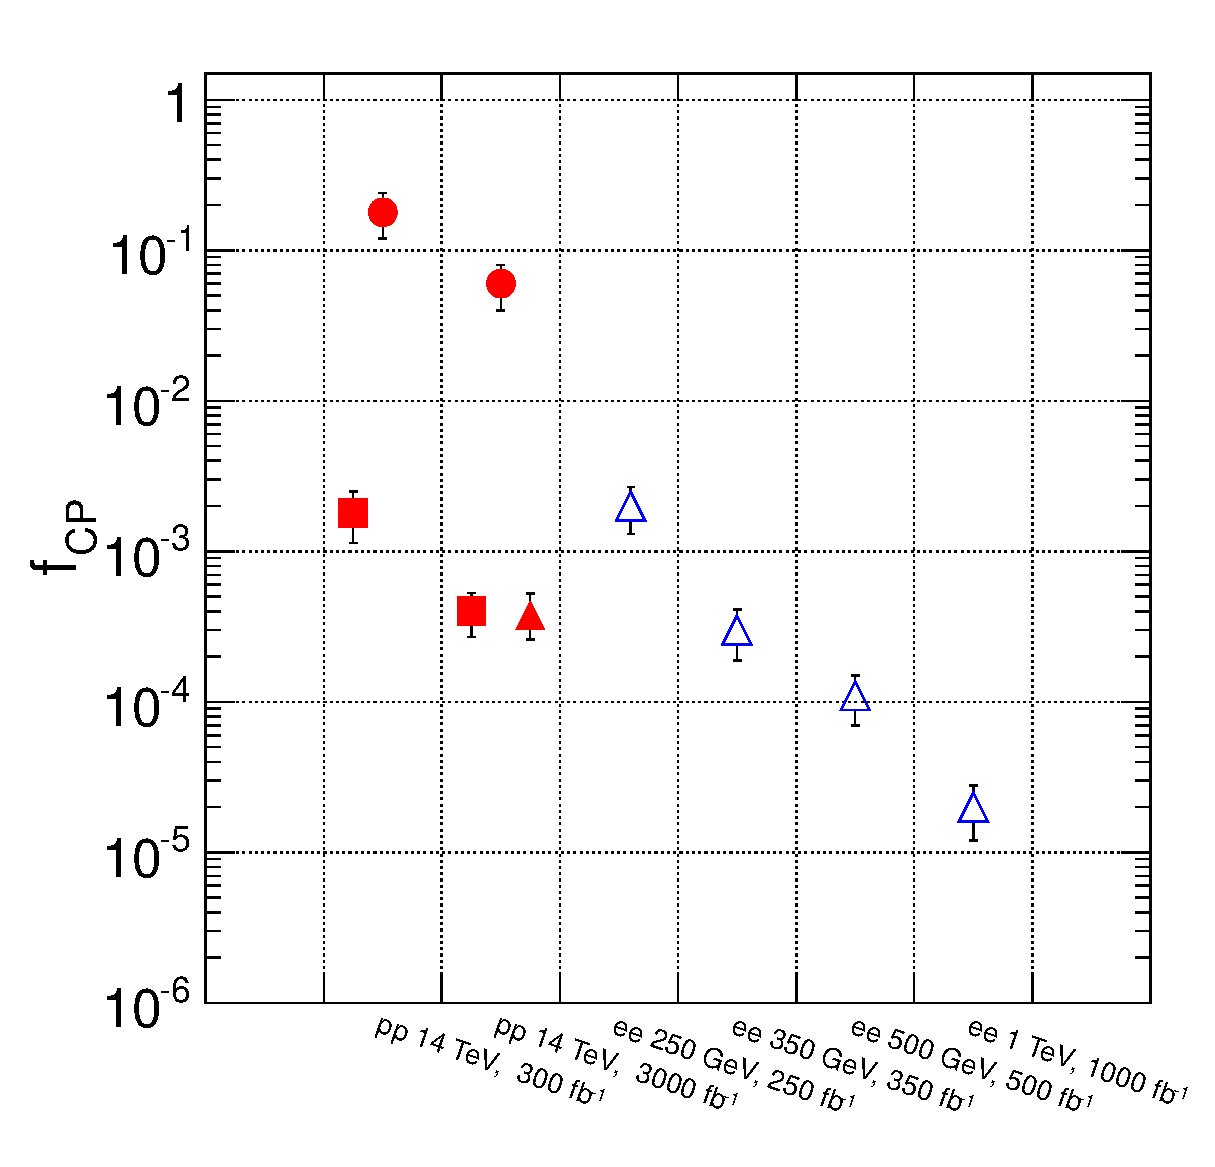
\includegraphics[width=.9\linewidth]{Conclusions/figures/summary_fcp}
\caption[Summary of Precisions for CP-Violating Anomalous Coupling in $HVV$ Vertex at LHC and Future Colliders]{Summary of $f_{CP}$ precisions on the $HVV$ vertex at the LHC (solid red) and proposed future colliders (open blue). VH (triangles) and VBF (square) production methods as well as $H\rightarrow VV$ decays (circles) are shown. Energies and luminosities are listed in the $x$-axis.}
\label{fig:SnowmassCP}
\end{center}
\end{figure}

At the time these sensitivities were projected, the off-shell measurement was not yet designed; these measurements are all from on-shell measurements. If we combine the off-shell anomalous coupling measurement techniques described in Sec.~\ref{sec:OffShellAnom}, the overall measurement of anomalous $HVV$ couplings can become even tighter, especially for VBF production. It is plausible that the sensitivity of $f_{CP}$ could become test some BSM theoretical predictions within the lifetime of the LHC. Until and unless the LHC observes new particles not predicted by the Standard Model, this technique and others like it can provide more concrete information concerning physics beyond the Standard Model.

By any standard, the searches and property measurements of the Higgs Boson should be considered a grand success, both for the Standard Model and the LHC. For their theoretical contribution, Higgs and Englert were jointly awarded the Nobel Prize in Physics in 2013. But the Higgs Boson was the last piece of the Standard Model which -- even with its immense predictive power and precision -- is known to be insufficient to explain all phenomena in particle physics. The next wave of searches, either through direct measurement of new particles or indirectly through precision Higgs boson properties, will aim to answer the current mysteries: What, exactly, is dark matter? What about dark energy? Why is there more matter than antimatter? In short, the question we must answer individually and cosmically: How did we get here and where are we going? That is the solitary goal of all particle physics, even physics in general. Through the LHC and the Higgs boson, we move closer to providing an answer.

